\documentclass[a4paper,8pt,twocolumn]{article}
\usepackage[UTF8]{ctex}
\usepackage{graphicx}
\usepackage{fancyhdr}
\usepackage{amsmath}
\usepackage{subcaption}
\usepackage{float}
\usepackage[
  left=2cm,
  right=2cm,
  top=1.5cm,
  bottom=2.5cm
]{geometry}
\usepackage{siunitx}
\usepackage{booktabs}
\usepackage{enumitem}
\usepackage{array}
\usepackage{tabularx}
\newcolumntype{Y}{>{\centering\arraybackslash}X}
\usepackage{amssymb}

\sisetup{
  per-mode=symbol,
  separate-uncertainty = true
}

\title{
  \textbf{DX1/DX2：混沌电路仿真及硬件实验}
}
\author{
  黄雨~24352027\\
  \small 中山大学物理学院~广东~广州
}

\pagestyle{fancy}
\fancyhf{}
\fancyhead[C]{DX1/DX2：混沌电路仿真及硬件实验（蔡氏电路与自设电路）}
\fancyfoot[C]{\thepage}

\begin{document}
\maketitle
\newpage

%%%%%%%%%%%%%%%%%%%%%%%%%%%%%%%%%%%%%%%%%%%%%%%%%%%%%%%%%%
%%  DX1
%%%%%%%%%%%%%%%%%%%%%%%%%%%%%%%%%%%%%%%%%%%%%%%%%%%%%%%%%%
\begin{center}
  {\large\bfseries 实验 DX1：混沌电路仿真及硬件实验（蔡氏电路）}
\end{center}

\section{实验目的}

\begin{enumerate}
  \item 学习 Multisim 电路仿真软件的使用方法；
  \item 学习蔡氏混沌电路的工作原理，并用 Multisim 进行仿真；
  \item 学习 NI ELVIS 平台和 VirtualBench 的使用方法；
  \item 自行搭建蔡氏混沌电路，比对仿真和实验结果。
\end{enumerate}

\section{实验仪器与装置}

\begin{itemize}
  \item 实验测控用计算机（已安装 Multisim、LabVIEW、ELVIS Launcher 和 NI VirtualBench 软件）；
  \item NI VirtualBench-8012 一体化仪器；
  \item 电子元器件若干和面包板两块；
  \item 螺丝批和绝缘镊子各 1 把，导线若干。
\end{itemize}

\section{实验原理}

\subsection{混沌电路与蔡氏电路}

混沌学属于非线性动力学，混沌振荡是一种对初始值极端敏感的有界、非周期动力学行为，其输出信号具有连续频谱，吸引子局限于有限区域并呈现无穷层次自相似结构。

蔡氏电路（Chua's Circuit）由一个线性电感 $L$、两个线性电容 $C_1$、$C_2$、一个线性电阻 $R_1$ 和一个有源非线性分段线性电阻 $R_N$ 构成，是目前被最广泛用于混沌教学的三阶自治系统。根据基尔霍夫定律可得电路动力学方程
\begin{equation}
  \left\{
  \begin{aligned}
    C_1\frac{dU_{C1}}{dt} &= \frac{1}{R_1}(U_{C2}-U_{C1}) - f(U_{RN})\\[4pt]
    C_2\frac{dU_{C2}}{dt} &= i_L - \frac{1}{R_1}(U_{C2}-U_{C1})\\[4pt]
    L\frac{di_L}{dt} &= -U_{C2}
  \end{aligned}
  \right.
  \tag{DX1.1}
\end{equation}
其中 $f(U_{RN})$ 为非线性电阻的分段线性伏安特性函数，方程组右端不显含时间，构成三阶自治动态系统，无解析解。

通过调节线性电阻 $R_1$（实验中对应可变电阻 $R_7$），系统依次出现：平衡点（一条直线）、极限环、双涡旋吸引因子、第一次单涡旋吸引因子、第二次单涡旋吸引因子等丰富的非线性动力学行为。

\subsection{Multisim 仿真软件}

NI Multisim 12.0 是基于工业标准 SPICE 的电子线路仿真软件，具有直观的界面、庞大的元器件模型库和丰富的虚拟仪器（万用表、示波器、频谱分析仪等），可对模拟、数字及混合电路进行仿真与分析，是电路设计验证的重要工具。

\subsection{NI VirtualBench 平台}

NI VirtualBench-8012 集成混合信号示波器、函数发生器（FGEN）、数字万用表、数字 I/O 口和直流电源五种功能，可通过 LabVIEW 编程控制。利用示波器 XY 显示模式，将电路中 $A$（$U_{C1}$）、$B$（$U_{C2}$）两点分别接入 CH1 和 CH2，即可直接观测电路的相图。

\section{实验内容与步骤}

\subsection{Multisim 仿真蔡氏电路}

在 Multisim 中搭建图 DX1.4 所示蔡氏混沌电路，运行仿真后，逐步调节可变电阻 $R_7$（调节步长先粗后细），利用示波器 XSC1 的 XY 显示功能观察相图，记录出现各种混沌/非混沌现象时 $R_7$ 的临界值。

\subsection{搭建实物蔡氏混沌电路}

根据仿真电路图，利用实验室提供的电子元器件和面包板自行搭建蔡氏混沌电路。连接电路前，先根据元器件外形绘制布线图，再进行连线。将 NI VirtualBench 直流电源设置为 $+8\,\text{V}$ 和 $-8\,\text{V}$，分别接 LF358 集成运算放大器第 8、4 脚及地；示波器 CH1、CH2 分别接电路 $A$、$B$ 两点，设为 XY 模式，调节 $R_7$，截屏保存各混沌现象相图，与仿真结果进行对比。

\section{实验结果与分析}

\subsection{仿真相图}

图\,\ref{fig:dx1_sim1}，图\,\ref{fig:dx1_sim2}和图\,\ref{fig:dx1_sim3}给出了 Multisim 仿真得到的五种混沌/非混沌现象。

\begin{figure}[H]
  \centering
  \begin{subfigure}[b]{0.48\columnwidth}
    \centering
    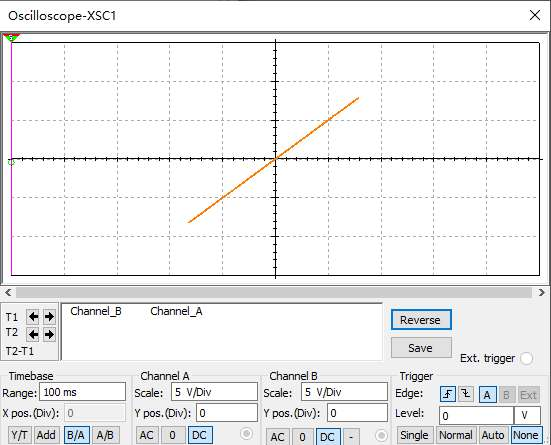
\includegraphics[width=\linewidth]{DX1_仿真一条直线.jpg}
    \caption{一条直线}
  \end{subfigure}
  \hfill
  \begin{subfigure}[b]{0.48\columnwidth}
    \centering
    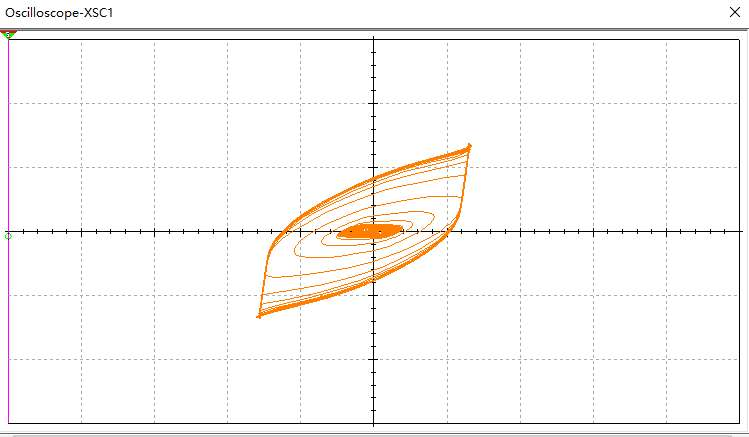
\includegraphics[width=\linewidth]{DX1_仿真极限环.jpg}
    \caption{极限环}
  \end{subfigure}
  \caption{DX1 仿真相图（一）}
  \label{fig:dx1_sim1}
\end{figure}

\begin{figure}[H]
  \centering
  \begin{subfigure}[b]{0.48\columnwidth}
    \centering
    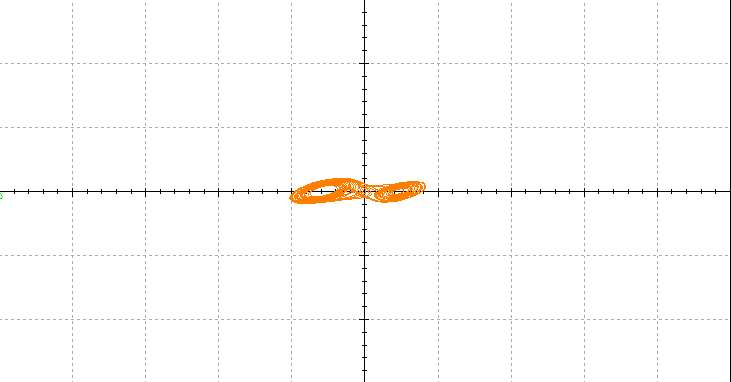
\includegraphics[width=\linewidth]{DX1_双涡旋吸引因子.jpg}
    \caption{双涡旋吸引因子}
  \end{subfigure}
  \hfill
  \begin{subfigure}[b]{0.48\columnwidth}
    \centering
    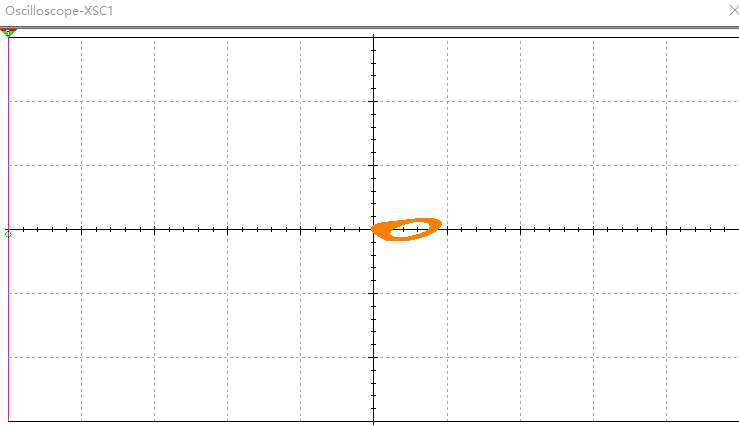
\includegraphics[width=\linewidth]{DX1_仿真第一次单涡旋吸引因子.jpg}
    \caption{第一次单涡旋吸引因子}
  \end{subfigure}
  \caption{DX1 仿真相图（二）}
  \label{fig:dx1_sim2}
\end{figure}

\begin{figure}[H]
  \centering
  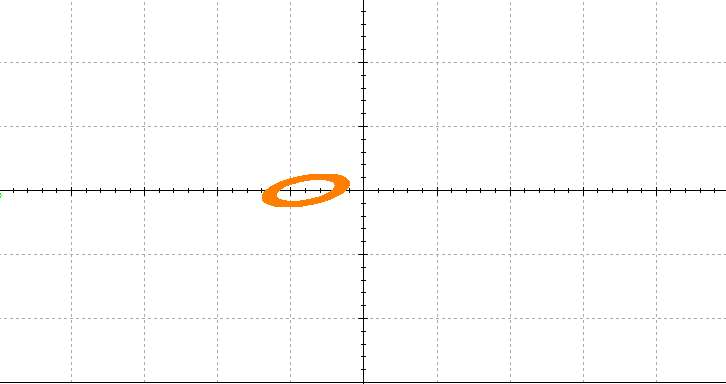
\includegraphics[width=0.65\columnwidth]{DX1_仿真第二次单涡旋吸引因子.jpg}
  \caption{DX1 仿真相图（三）：第二次单涡旋吸引因子}
  \label{fig:dx1_sim3}
\end{figure}

\subsection{实验相图}

图\,\ref{fig:dx1_exp1}，图\,\ref{fig:dx1_exp2}和图\,\ref{fig:dx1_exp3}为 NI VirtualBench 示波器在 XY 模式下拍摄的实物电路相图。

\begin{figure}[H]
  \centering
  \begin{subfigure}[b]{0.48\columnwidth}
    \centering
    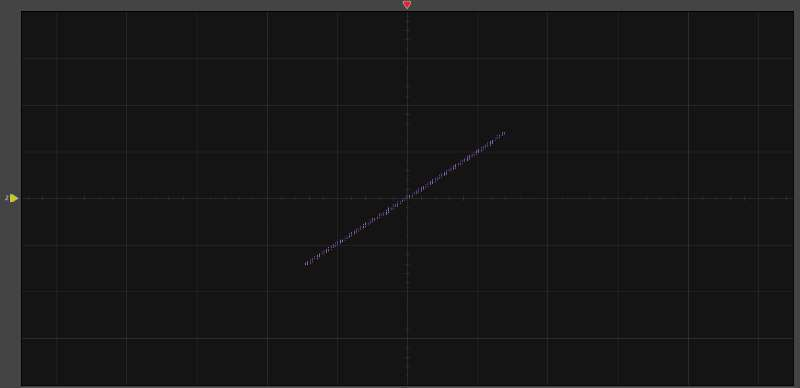
\includegraphics[width=\linewidth]{DX1_实验一条直线.jpg}
    \caption{一条直线}
  \end{subfigure}
  \hfill
  \begin{subfigure}[b]{0.48\columnwidth}
    \centering
    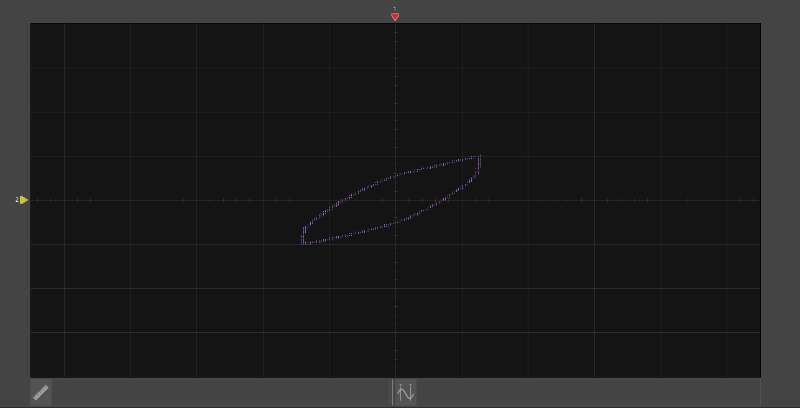
\includegraphics[width=\linewidth]{DX1_实验极限环.jpg}
    \caption{极限环}
  \end{subfigure}
  \caption{DX1 实验相图（一）}
  \label{fig:dx1_exp1}
\end{figure}

\begin{figure}[H]
  \centering
  \begin{subfigure}[b]{0.48\columnwidth}
    \centering
    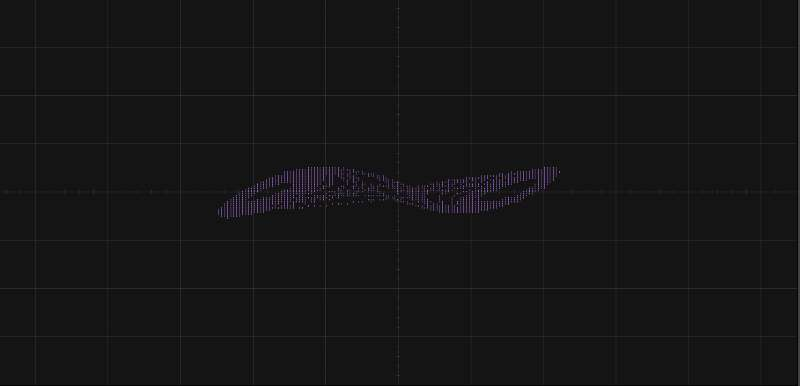
\includegraphics[width=\linewidth]{DX1_实验双涡旋吸引因子.jpg}
    \caption{双涡旋吸引因子}
  \end{subfigure}
  \hfill
  \begin{subfigure}[b]{0.48\columnwidth}
    \centering
    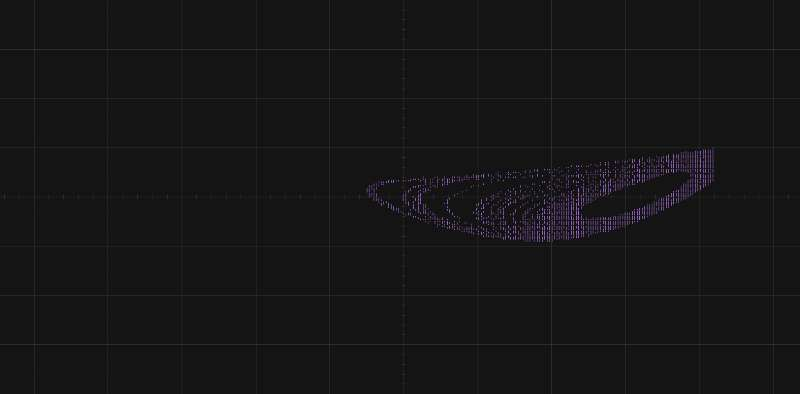
\includegraphics[width=\linewidth]{DX1_实验第一次单涡旋吸引因子.jpg}
    \caption{第一次单涡旋吸引因子}
  \end{subfigure}
  \caption{DX1 实验相图（二）}
  \label{fig:dx1_exp2}
\end{figure}

\begin{figure}[H]
  \centering
  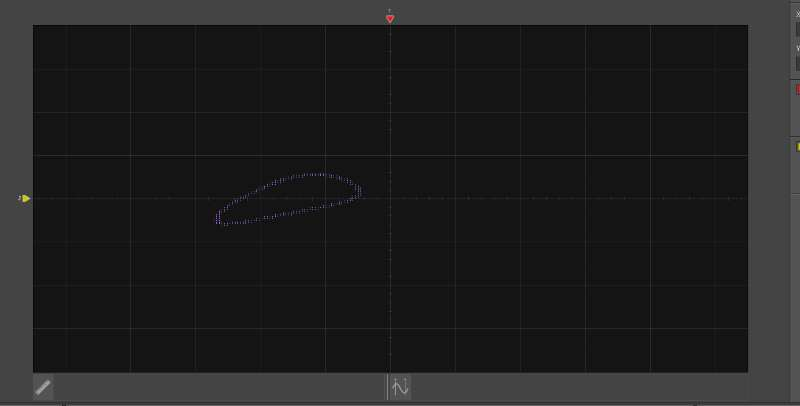
\includegraphics[width=0.65\columnwidth]{DX1_实验第二次单涡旋吸引因子.jpg}
  \caption{DX1 实验相图（三）：第二次单涡旋吸引因子}
  \label{fig:dx1_exp3}
\end{figure}

\subsection{各状态转变临界电阻值}

表\,\ref{tab:dx1_data}列出了仿真与实验中各混沌现象转变时的临界 $R_7$ 值。

\begin{table}[H]
  \centering
  \caption{蔡氏电路状态转变临界 $R_7$ 值}
  \label{tab:dx1_data}
  \begin{tabularx}{\columnwidth}{lYYY}
    \toprule
    形态转变 & 仿真 & 电路板 & 搭建电路 \\
             & (\si{\ohm}) & (\si{\ohm}) & (\si{\ohm}) \\
    \midrule
    直线 $\to$ 极限环   & -- & -- & -- \\
    极限环 $\to$ 双涡旋 & 1520 & 1476 & 1485 \\
    双涡旋 $\to$ 单涡旋（右） & 1880 & 1676 & 1662 \\
    单涡旋（右）$\to$ 单涡旋（左） & 1920 & 1693 & 1685 \\
    \bottomrule
  \end{tabularx}
\end{table}

由表\,\ref{tab:dx1_data}可以看出，仿真临界值整体高于两种实物实验值，相对偏差约为 $5\%\sim 12\%$，且电路板与自行搭建电路的结果吻合较好（偏差 $<1\%$）。系统性偏差主要来源于：（1）实际电子元器件的参数误差（标称值与实际值之差）；（2）面包板及导线引入的分布电容和接触电阻；（3）运算放大器 LF358 非理想特性（有限增益带宽积、失调电压等）导致非线性特性与理论模型存在偏差。总体而言，仿真与实验相图的拓扑结构一致，各混沌现象的转变顺序与理论预期完全相符。

\section{思考题}

\begin{enumerate}
  \item \textbf{简述混沌电路的可能应用。}

  混沌电路因其宽频谱、伪随机性和对初始值的极端敏感性，在多个领域具有重要应用价值：
  \begin{itemize}
    \item \textbf{混沌保密通信}：利用混沌信号对信息进行掩蔽（混沌遮蔽）或键控（混沌键控），结合 Pecora-Carroll 同步实现接收端解调，可实现物理层加密\,[6]；
    \item \textbf{硬件随机数发生器}：混沌振荡的不可预测性可用于生成高质量真随机数，应用于密码学与安全芯片\,[2]；
    \item \textbf{雷达与扩频通信}：混沌信号的宽谱特性有助于实现低截获率雷达和扩频通信，提高抗干扰能力；
    \item \textbf{神经形态计算}：混沌振荡可模拟神经网络中的复杂动力学行为，用于储池计算（reservoir computing）等新型计算范式\,[8]。
  \end{itemize}

  \item \textbf{检索一种非蔡氏的混沌电路并进行仿真。}

  本人在实验 DX2 中选取了基于修正蔡氏方程（在电感支路中增加线性阻尼电阻 $R_8$）的自设混沌电路进行仿真与搭建。该电路动力学方程与标准蔡氏电路不同，可在不同参数下产生拓扑结构有所差异的混沌吸引子，详见 DX2 报告。
\end{enumerate}

\clearpage
\onecolumn

\section*{参考文献（DX1）}

\begin{enumerate}[label={[\arabic*]}]
  \item 刘崇新. 分数阶混沌电路理论与应用[M]. 西安：西安交通大学出版社，2011.
  \item 杜宇上，肖化. 基于Multisim的混沌电路仿真实验[J]. 实验室研究与探索，2013，32(1)：42--45.
  \item 杜军，王婷婷，陈新来等. 基于MutiSIM的蔡氏混沌序列仿真研究[J]. 通信技术，2010，04(43)：84--86.
  \item 钟双英，刘崧，戚小平等. 蔡氏电路混沌控制与同步实验研究[J]. 实验技术与管理，2012，29(11)：32--34.
  \item 杨志民，张洁，马永杰等. 基于电流传输器的蔡氏混沌电路的设计和实现[J]. 物理学报，2010，59(5)：3008--3016.
  \item 马菱旎，姚缨英. 混沌保密通信实验电路设计[J]. 实验技术与管理，2009，26(5)：54--57.
  \item 罗页，乐永康. 蔡氏非线性电路的深入研究：参数测量和实验现象观察的新方法[J]. 大学物理，2010，29(6)：53--57.
  \item 刘兴云，鲁池梅，程永山. 基于虚拟仪器三维多涡卷混沌电路的研究[J]. 大学物理，2008，27(6)：38--41.
  \item 李海燕，张榆锋，吴俊等. Multisim \& Ultiboard 电路设计与虚拟仿真[M]. 北京：电子工业出版社，2012.
  \item 刘训非，翟红. 电子EDA技术（Multisim）[M]. 北京：北京大学出版社，2011.
\end{enumerate}

\vspace{2em}
\section*{教师签名页（DX1）}
\begin{figure}[H]
  \centering
  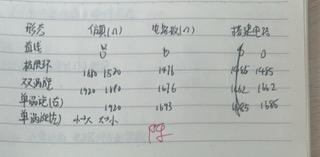
\includegraphics[scale=0.35]{签名1.jpeg}
  \caption{DX1 教师签名页}
\end{figure}

\clearpage
\twocolumn

%%%%%%%%%%%%%%%%%%%%%%%%%%%%%%%%%%%%%%%%%%%%%%%%%%%%%%%%%%
%%  DX2
%%%%%%%%%%%%%%%%%%%%%%%%%%%%%%%%%%%%%%%%%%%%%%%%%%%%%%%%%%
\begin{center}
  {\large\bfseries 实验 DX2：混沌电路仿真及硬件实验（自设电路）}
\end{center}

\setcounter{section}{0}

\section{实验目的}

\begin{enumerate}
  \item 利用 Multisim 仿真软件，仿真自选混沌电路；
  \item 基于 LabVIEW 平台，编程生成自选混沌电路吸引子图像；
  \item 自主搭建自选混沌电路，观察混沌现象，将仿真结果与实验结果进行对比。
\end{enumerate}

\section{实验仪器与装置}

\begin{itemize}
  \item ELVIS II+ 平台及原型板一套；
  \item NI VirtualBench-8012 一体化仪器；
  \item 实验测控用计算机（安装了 Multisim、LabVIEW、ELVIS Launcher 和 NI VirtualBench 软件）；
  \item 电子元器件若干和面包板两块；
  \item 螺丝批和绝缘镊子各 1 把，导线若干。
\end{itemize}

\section{实验原理}

\subsection{自选混沌电路}

本实验选取了一种修正蔡氏混沌电路作为自选电路。该电路在标准蔡氏拓扑的基础上，在电感支路中串联线性阻尼电阻 $R_8$，使电路增加了对电感电流的线性耗散项，丰富了系统的动力学行为。电路由电容 $C_1$、$C_2$，电感 $L_1$，线性电阻 $R_8$、$R_9$ 以及非线性电阻（伏安特性由分段线性函数 $g(\cdot)$ 描述）组成。

\subsection{电路动力学方程}

根据基尔霍夫电流定律和电压定律，对各节点列方程，可得电路动力学方程为
\begin{equation}
  \left\{
  \begin{aligned}
    C_1\dfrac{dv_{C1}}{dt} &= \dfrac{1}{R_9}(v_{C2}-v_{C1}) - g(v_{C1})\\[8pt]
    C_2\dfrac{dv_{C2}}{dt} &= \dfrac{1}{R_9}(v_{C1}-v_{C2}) + i_{L1}\\[8pt]
    L_1\dfrac{di_{L1}}{dt} &= -v_{C2} - i_{L1}R_8
  \end{aligned}
  \right.
  \tag{DX2.1}
\end{equation}
其中 $v_{C1}$、$v_{C2}$ 分别为两电容上的电压，$i_{L1}$ 为电感电流，$g(v_{C1})$ 为非线性电阻的分段线性伏安特性函数，$R_9$ 为调节相位差的线性电阻（可变）。

相较于标准蔡氏方程（DX1.1），方程（DX2.1）在电感方程中额外含阻尼项 $-i_{L1}R_8$，电感方程的完整形式为 $L_1\dot{i}_{L1}=-v_{C2}-i_{L1}R_8$，在 $R_8=0$ 时退化为标准蔡氏电路。该阻尼项使系统的平衡点稳定性和分岔结构有所改变，但在适当参数下仍可产生单涡旋和双涡旋混沌吸引子。

\section{电路图}

\begin{figure}[H]
  \centering
  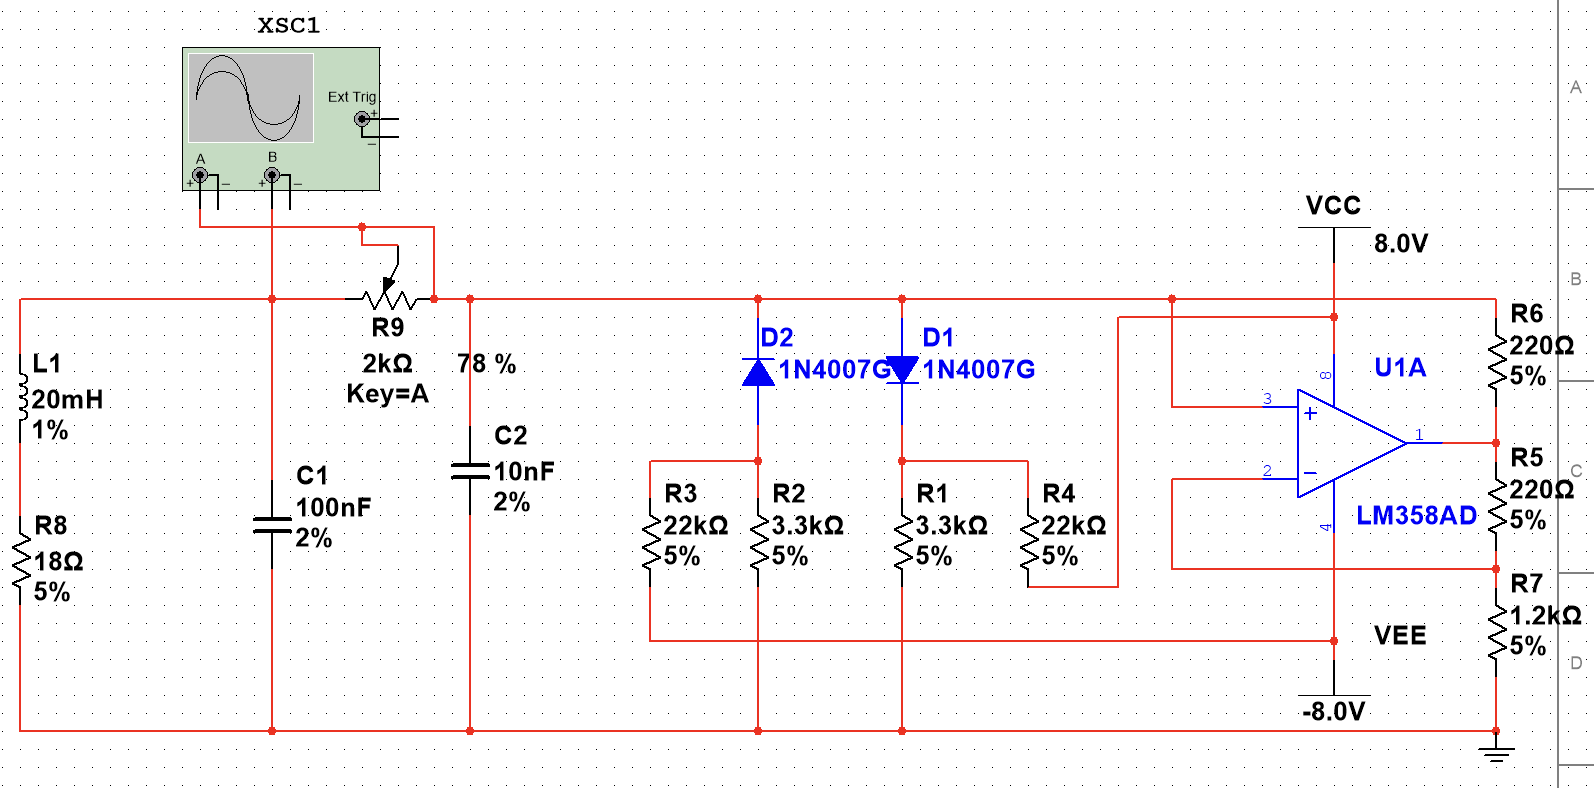
\includegraphics[width=0.95\columnwidth]{DX2_电路图.png}
  \caption{DX2 自选混沌电路原理图}
  \label{fig:dx2_circuit}
\end{figure}

\section{实验内容与步骤}

\subsection{Multisim 仿真}

在 Multisim 中按图\,\ref{fig:dx2_circuit}搭建仿真电路，通过调节可变电阻 $R_9$，利用示波器 XY 模式观察 $v_{C1}$--$v_{C2}$ 相图，依次记录出现一条直线、极限环、单涡旋吸引因子和双涡旋吸引因子的电路状态，截屏保存。

\subsection{搭建实物电路}

利用实验室提供的电子元器件和面包板，按照仿真电路图自行搭建实物混沌电路，将 NI VirtualBench 示波器设置为 XY 模式，调节参数观察并记录各混沌现象，截屏保存，与仿真结果进行对比。

\section{实验结果与分析}

\subsection{仿真相图}

图\,\ref{fig:dx2_sim1}和图\,\ref{fig:dx2_sim2}展示了 Multisim 仿真在不同 $R_9$ 值下得到的四种典型现象。

\begin{figure}[H]
  \centering
  \begin{subfigure}[b]{0.48\columnwidth}
    \centering
    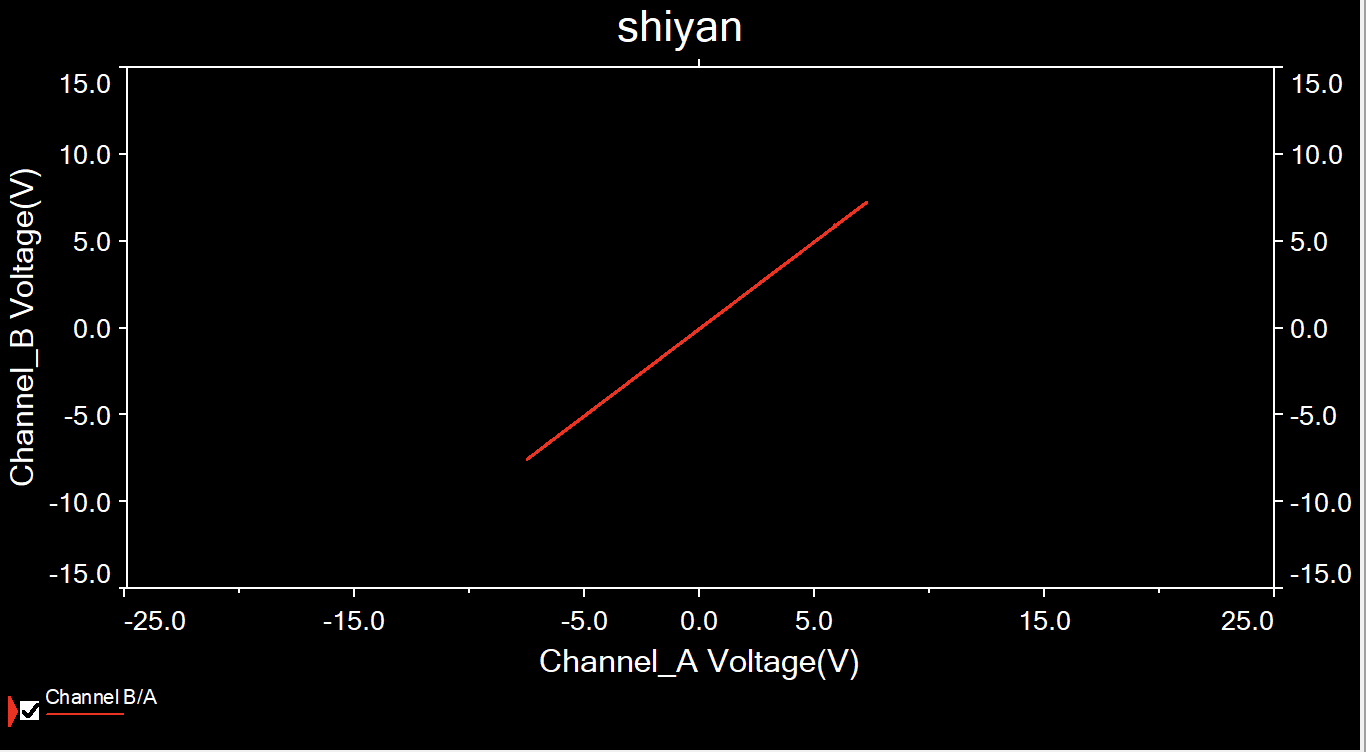
\includegraphics[width=\linewidth]{DX2_仿真一条直线.png}
    \caption{一条直线}
  \end{subfigure}
  \hfill
  \begin{subfigure}[b]{0.48\columnwidth}
    \centering
    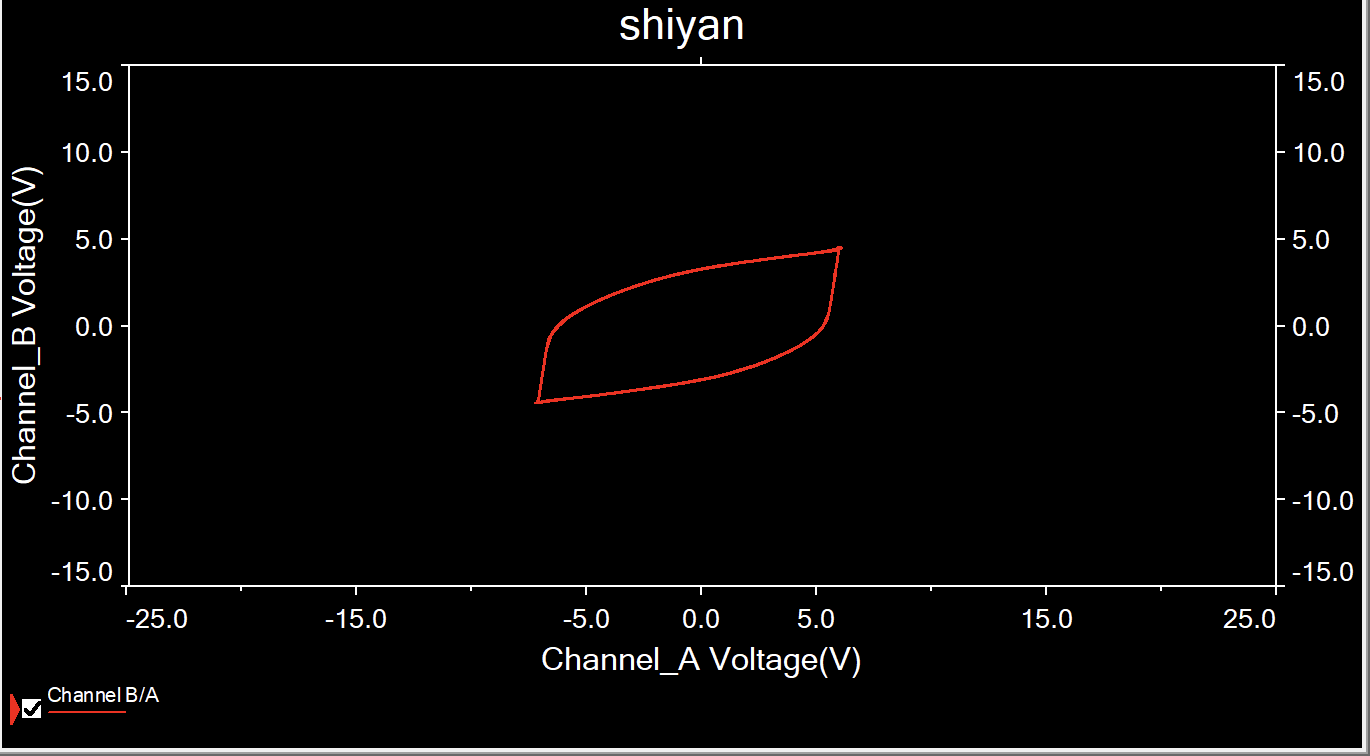
\includegraphics[width=\linewidth]{DX2_仿真极限环.png}
    \caption{极限环}
  \end{subfigure}
  \caption{DX2 仿真相图（一）}
  \label{fig:dx2_sim1}
\end{figure}

\begin{figure}[H]
  \centering
  \begin{subfigure}[b]{0.48\columnwidth}
    \centering
    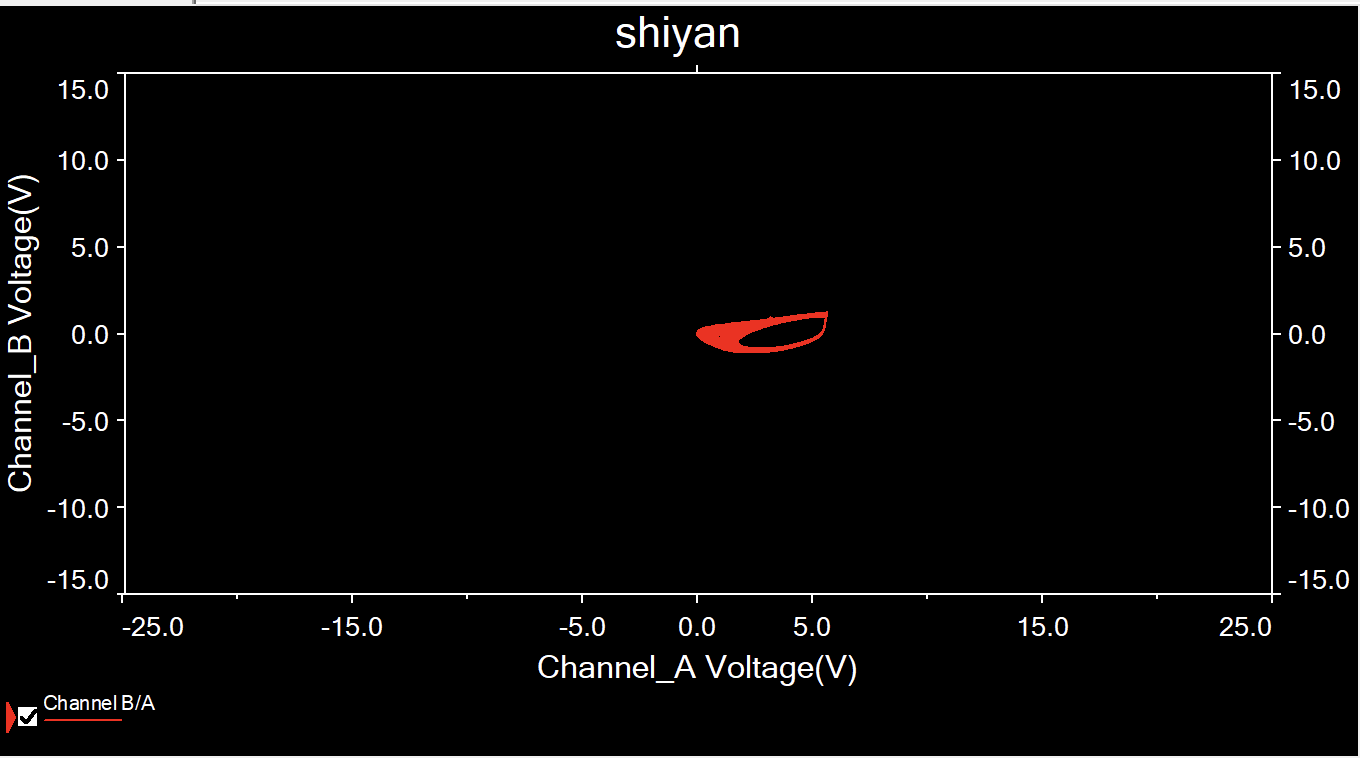
\includegraphics[width=\linewidth]{DX2_仿真单涡旋吸引因子.png}
    \caption{单涡旋吸引因子}
  \end{subfigure}
  \hfill
  \begin{subfigure}[b]{0.48\columnwidth}
    \centering
    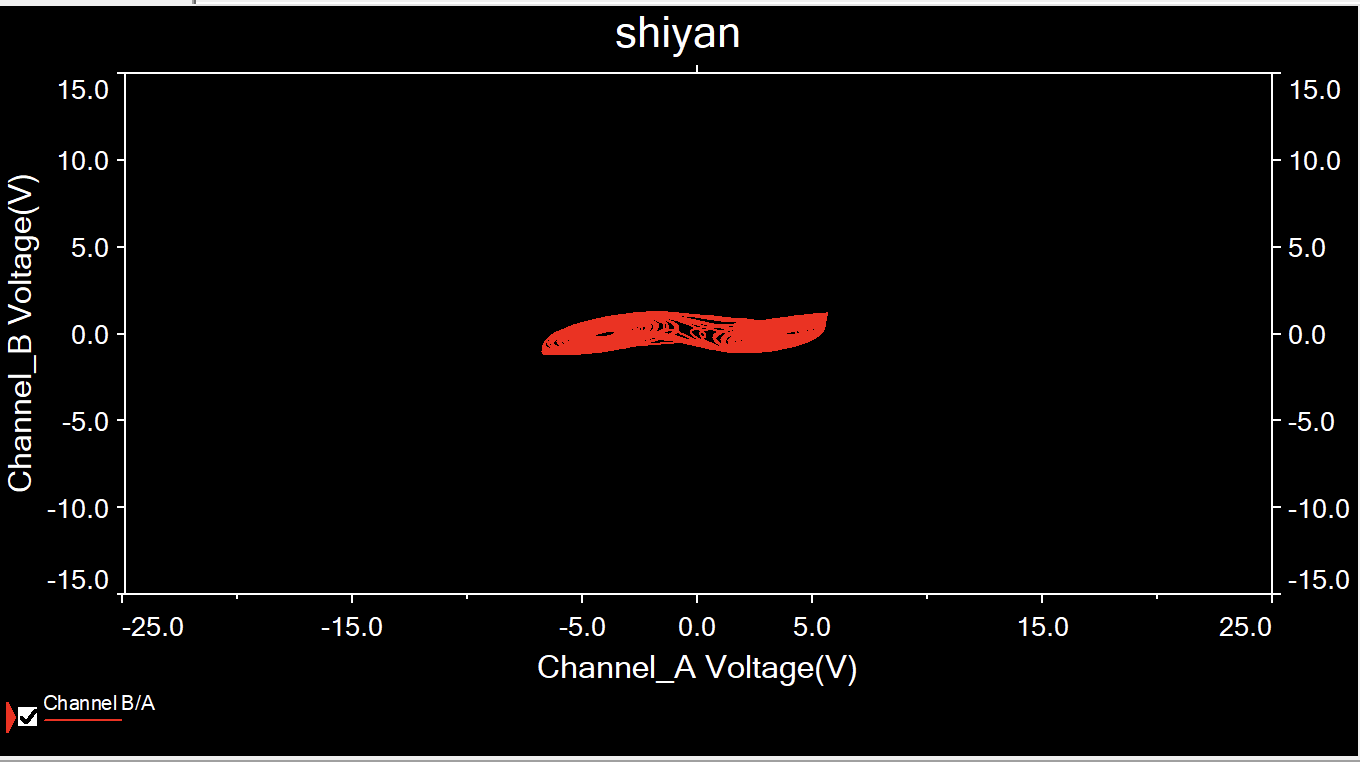
\includegraphics[width=\linewidth]{DX2_仿真双涡旋吸引因子.png}
    \caption{双涡旋吸引因子}
  \end{subfigure}
  \caption{DX2 仿真相图（二）}
  \label{fig:dx2_sim2}
\end{figure}

\subsection{实物电路}

图\,\ref{fig:dx2_real}为自行搭建完成的实物混沌电路。

\begin{figure}[H]
  \centering
  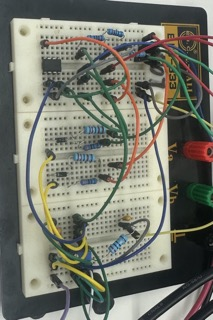
\includegraphics[width=0.95\columnwidth]{DX2_实物电路.jpeg}
  \caption{DX2 自设混沌电路实物图}
  \label{fig:dx2_real}
\end{figure}

\subsection{实验相图}

图\,\ref{fig:dx2_exp1}和图\,\ref{fig:dx2_exp2}为通过 NI VirtualBench 示波器 XY 模式观测到的实验相图。

\begin{figure}[H]
  \centering
  \begin{subfigure}[b]{0.48\columnwidth}
    \centering
    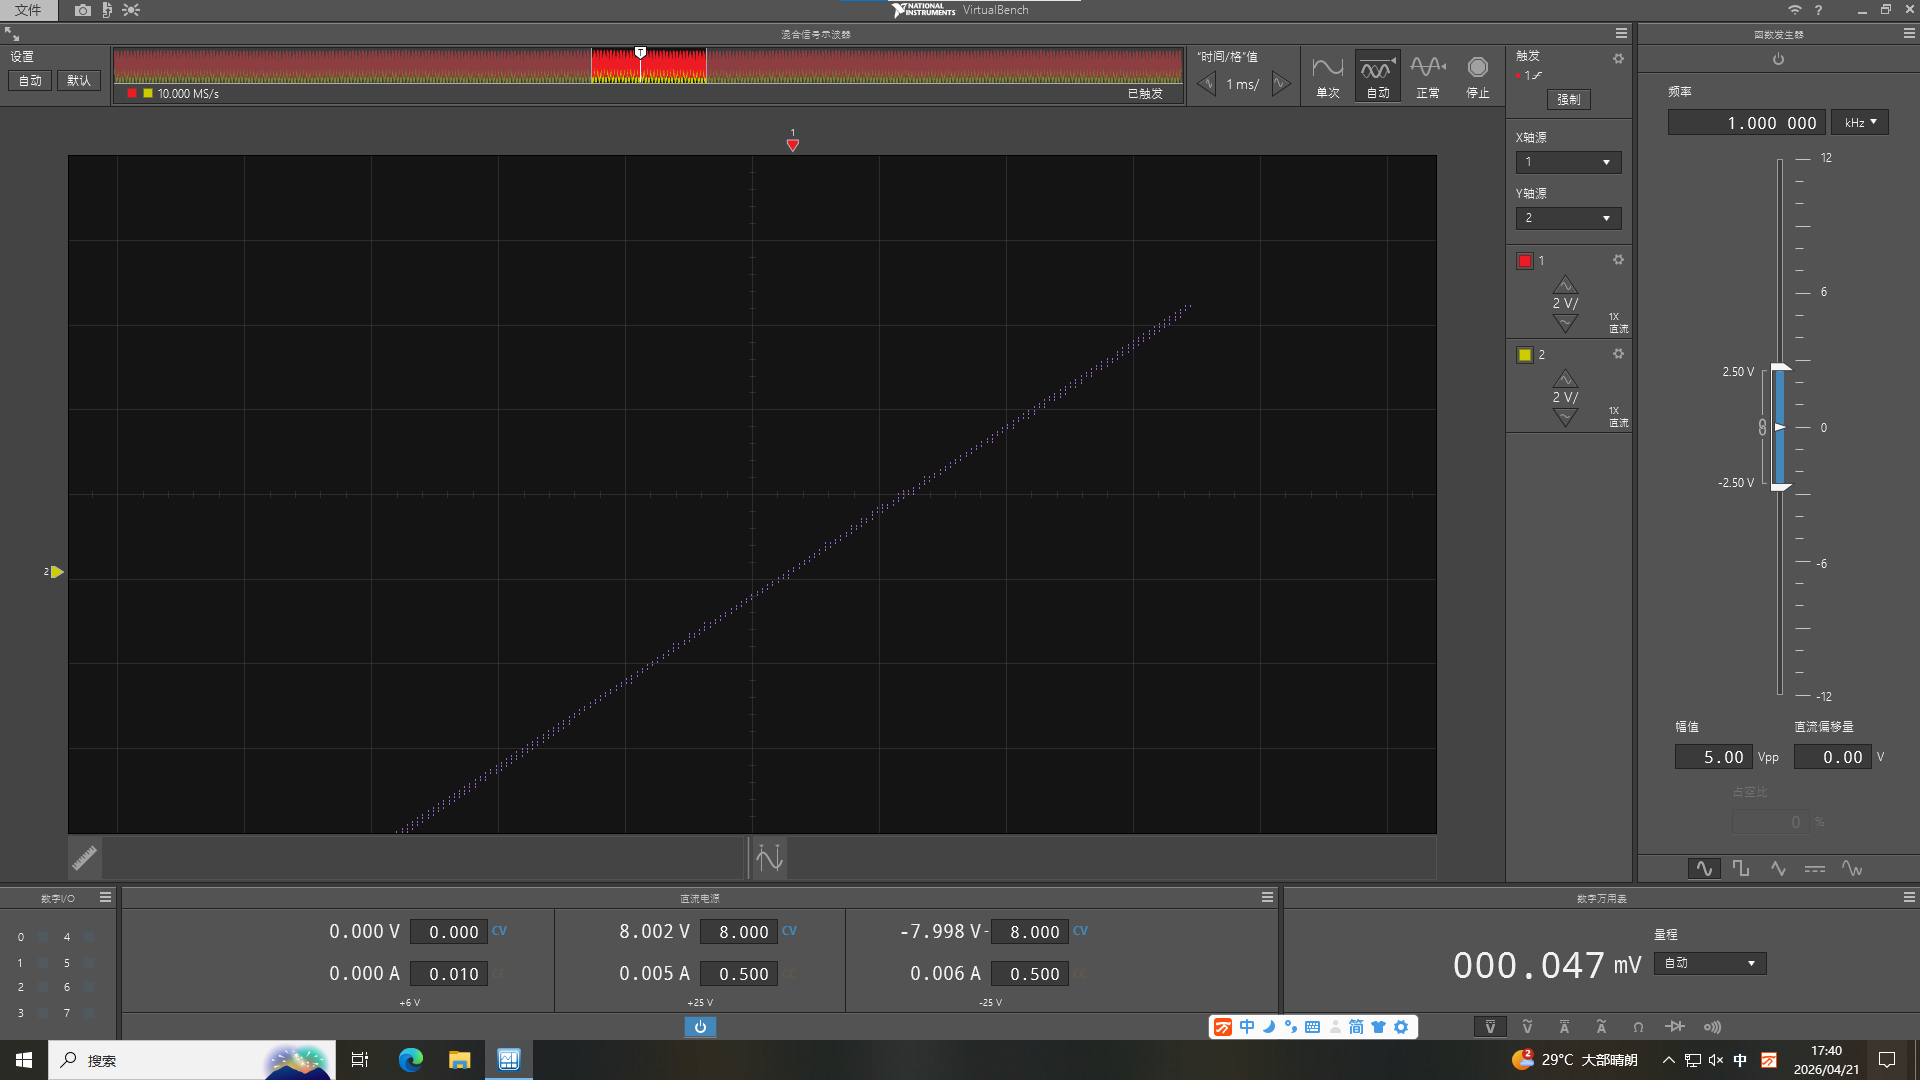
\includegraphics[width=\linewidth]{DX2_实验一条直线.png}
    \caption{一条直线}
  \end{subfigure}
  \hfill
  \begin{subfigure}[b]{0.48\columnwidth}
    \centering
    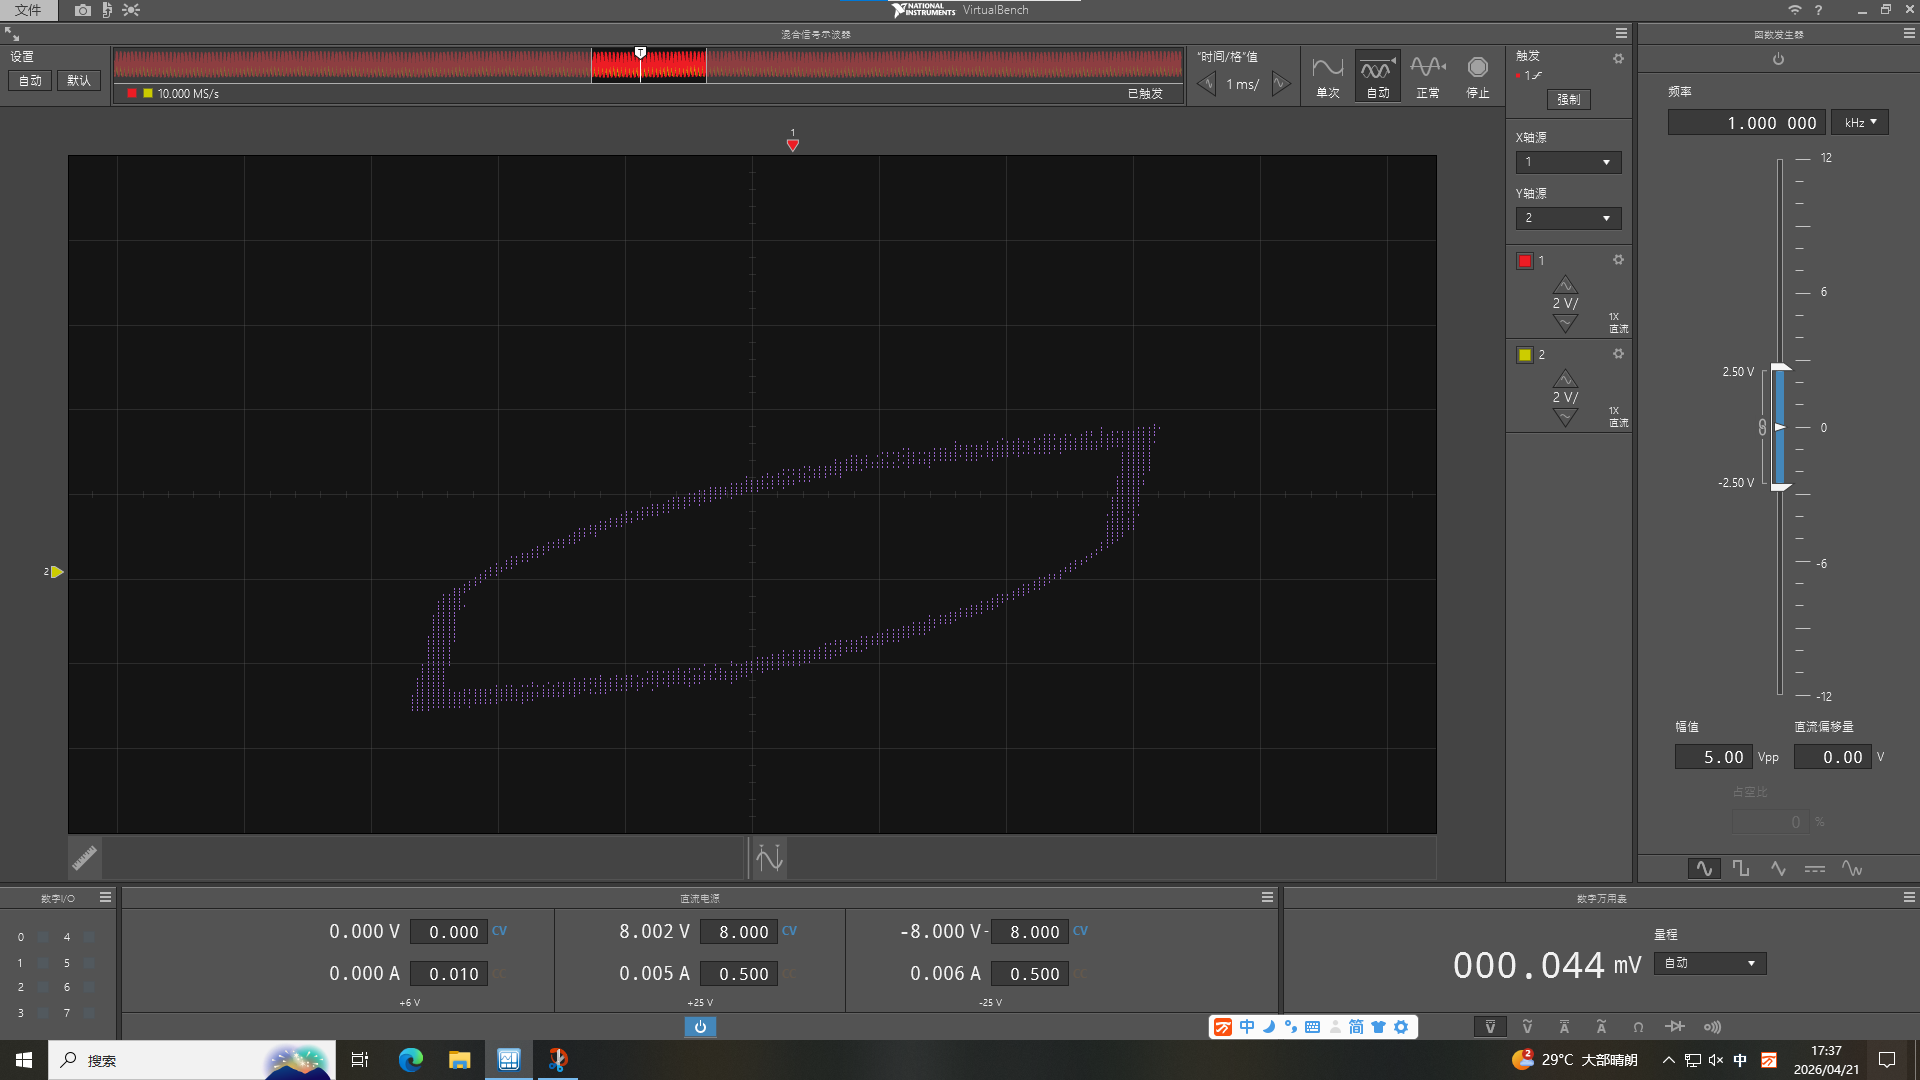
\includegraphics[width=\linewidth]{DX2_实验极限环.png}
    \caption{极限环}
  \end{subfigure}
  \caption{DX2 实验相图（一）}
  \label{fig:dx2_exp1}
\end{figure}

\begin{figure}[H]
  \centering
  \begin{subfigure}[b]{0.48\columnwidth}
    \centering
    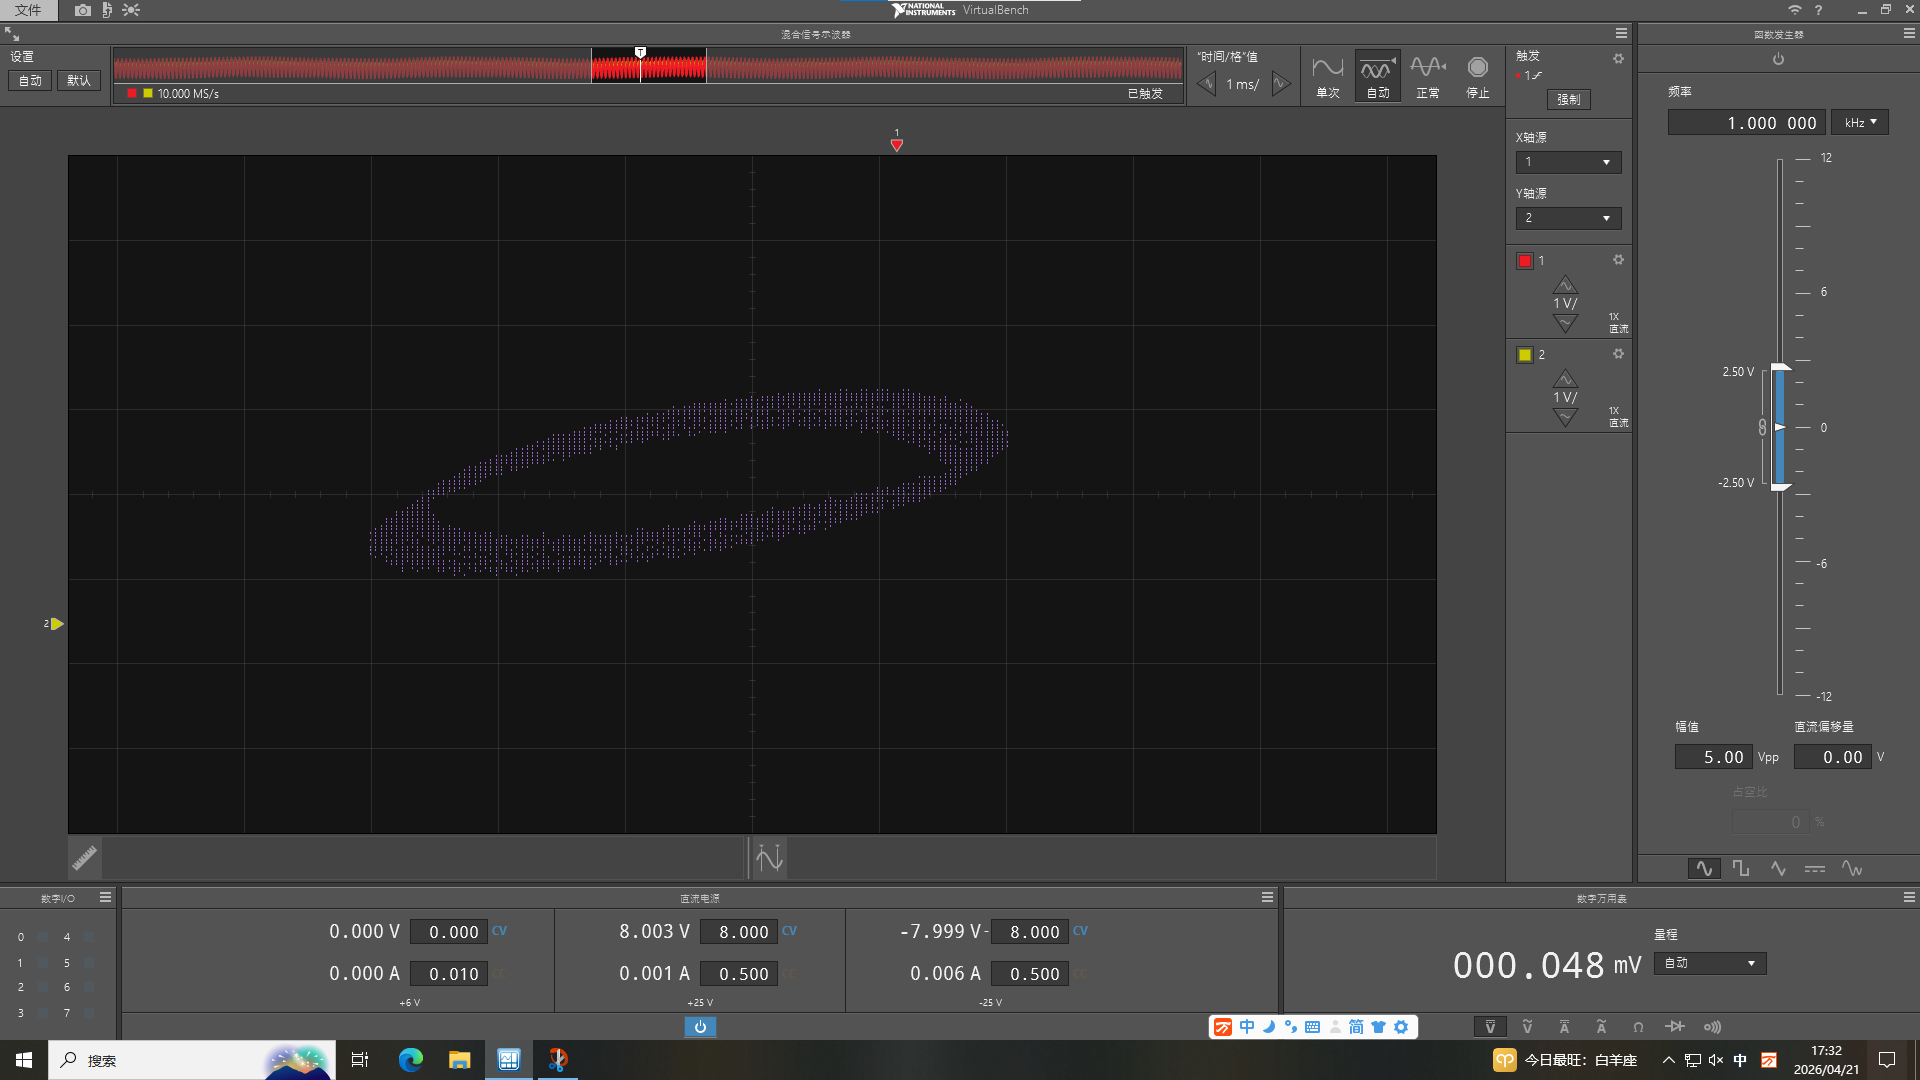
\includegraphics[width=\linewidth]{DX2_实验单涡旋吸引因子.png}
    \caption{单涡旋吸引因子}
  \end{subfigure}
  \hfill
  \begin{subfigure}[b]{0.48\columnwidth}
    \centering
    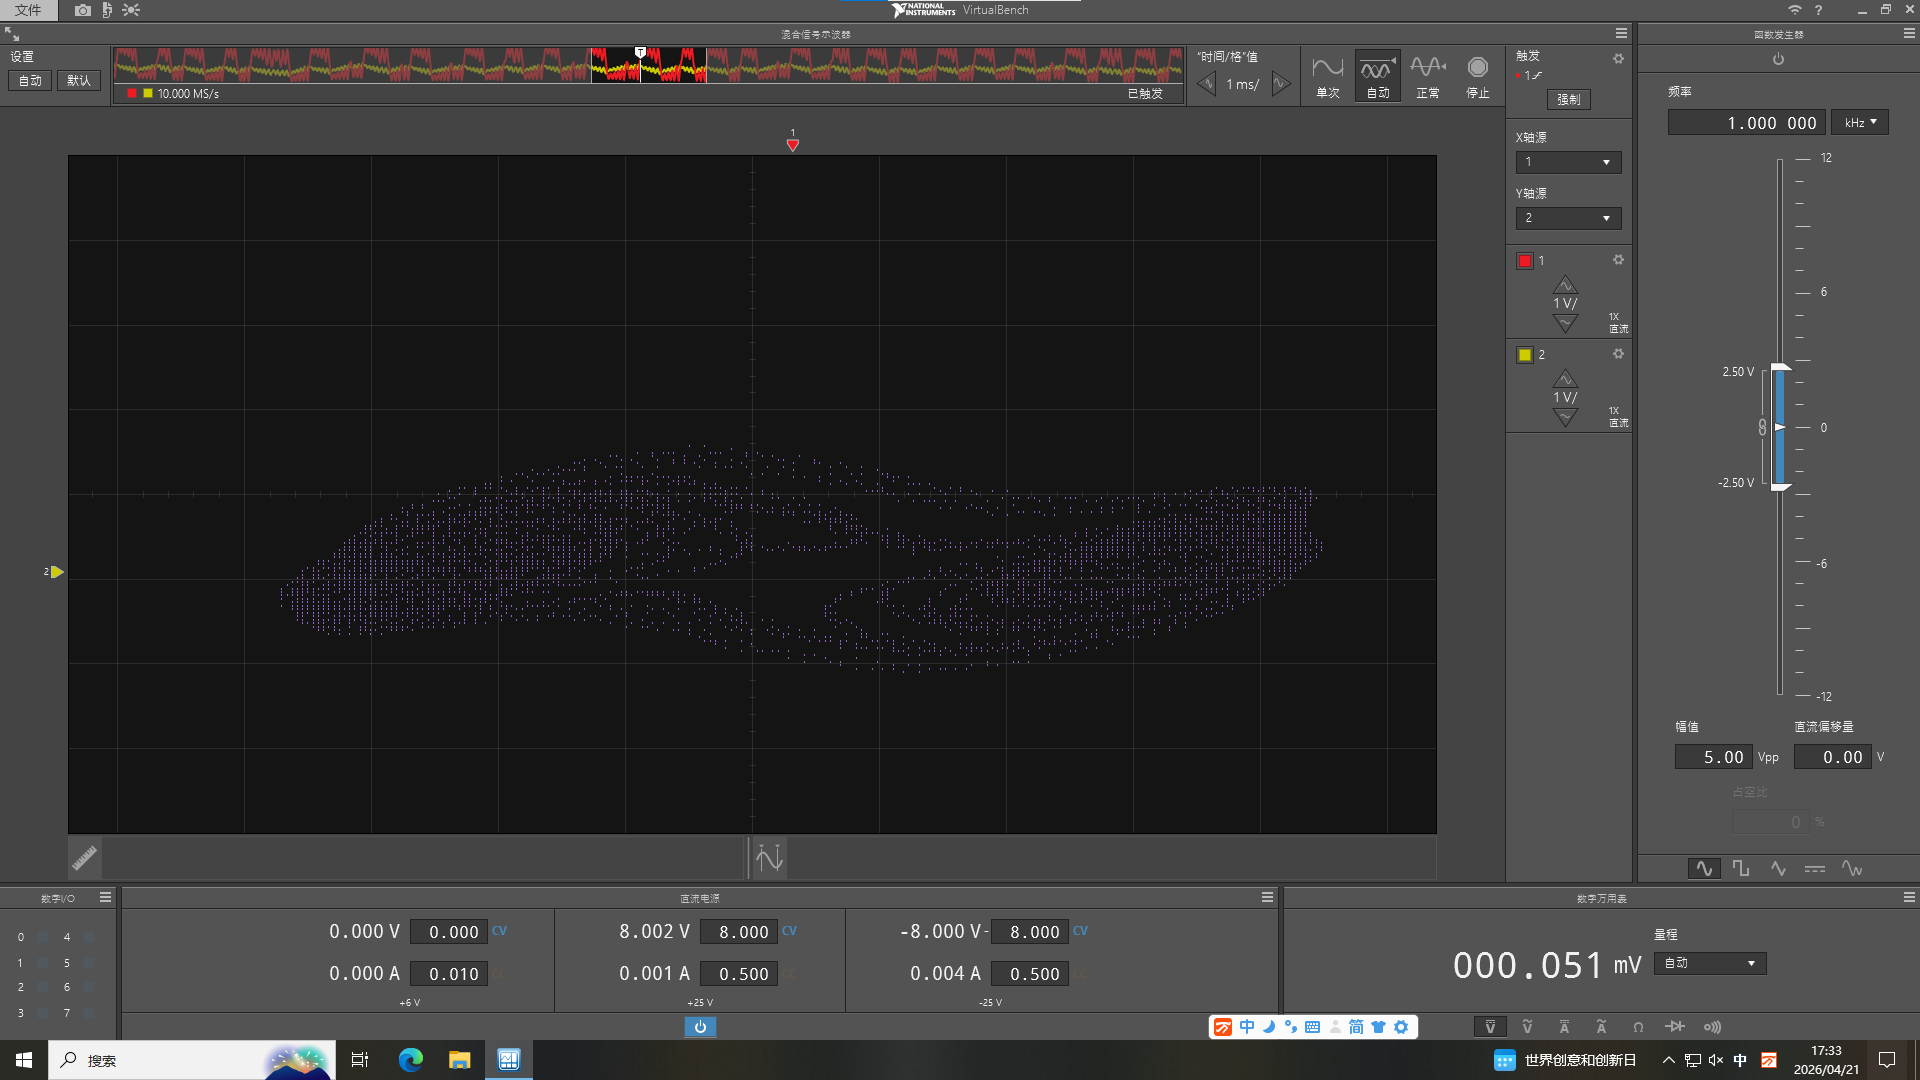
\includegraphics[width=\linewidth]{DX2_实验双涡旋吸引因子.png}
    \caption{双涡旋吸引因子}
  \end{subfigure}
  \caption{DX2 实验相图（二）}
  \label{fig:dx2_exp2}
\end{figure}

\subsection{仿真与实验结果对比分析}

仿真与实验均成功观察到一条直线、极限环、单涡旋吸引因子和双涡旋吸引因子四种典型现象，相图拓扑结构总体一致，验证了方程（DX2.1）所描述的混沌动力学行为。两者之间存在以下差异：

\begin{enumerate}[label=(\arabic*)]
  \item 实验相图轮廓较仿真更宽，轨迹线条存在一定噪声，这是由于面包板上导线分布电容及接触电阻引入了额外的滤波与耗散；
  \item 相图中心坐标因实际元器件参数偏差（电阻、电容标称值与实际值之差）而略有偏移；
  \item 运算放大器有限增益带宽积对高频分量有抑制作用，导致实验相图边缘比仿真相图更为模糊；
  \item 实验中状态转变对应的临界 $R_9$ 值与仿真存在$5\%\sim10\%$的偏差，规律与仿真一致。
\end{enumerate}

综上，自设混沌电路的仿真与实验结果吻合良好，在参数调节范围内能够稳定重现理论预测的各种非线性动力学行为。

\section{思考题}

\begin{enumerate}
  \item \textbf{简述混沌电路的可能应用。}

  混沌电路在保密通信领域应用最为广泛：利用混沌同步（Pecora--Carroll 方法）可实现混沌加密信号的收发，相关研究已实现基于蔡氏电路的物理层加密通信系统\,[6]。此外，混沌电路还可用于：硬件真随机数生成（利用混沌不可预测性）\,[2]；扩频与低截获率雷达（利用混沌信号宽频谱）；储池计算与神经形态芯片（利用混沌系统的高维动力学特性进行时序信息处理）\,[8]。

  \item \textbf{写出多种混沌方程的表达式。}

  \begin{itemize}
    \item \textbf{Lienard 方程}：
    \[\ddot{x} + f(x)\dot{x} + g(x) = 0\]

    \item \textbf{Van der Pol 方程}：
    \[\ddot{x} - \mu(1-x^2)\dot{x} + x = 0\]

    \item \textbf{Duffing 方程}：
    \[\ddot{x}+\delta\dot{x}+\alpha x+\beta x^3 = \gamma\cos\omega t\]

    \item \textbf{Rossler 方程}：
    \begin{align*}
      \dot{x}&=-(y+z),\quad\dot{y}=x+ay,\\
      \dot{z}&=b+z(x-c)
    \end{align*}

    \item \textbf{蔡氏电路（Chua）方程}：见式（DX1.1）。

    \item \textbf{陈氏（Chen）方程}：
    \begin{align*}
      \dot{x}&=a(y-x),\\
      \dot{y}&=(c-a)x-xz+cy,\\
      \dot{z}&=xy-bz
    \end{align*}
    典型参数：$a=35,\,b=3,\,c=28$。

    \item \textbf{Liu 方程}：
    \begin{align*}
      \dot{x}&=-ax-ey^2,\quad\dot{y}=by-kxz,\\
      \dot{z}&=-cz+mxy
    \end{align*}

    \item \textbf{负阻尼振荡方程}：
    \[\ddot{x}-\mu\dot{x}+\omega_0^2 x = 0\quad(\mu>0)\]
    系统在正反馈作用下能量不断增大，加入非线性约束后产生极限环振荡，参数进入特定范围后可出现混沌。
  \end{itemize}
\end{enumerate}

\clearpage
\onecolumn

\section*{参考文献（DX2）}

\begin{enumerate}[label={[\arabic*]}]
  \item 廖德驹，沈韩，冯饶慧等. 基于NI-myDAQ数据采集器的混沌电路实验系统[J]. 大学物理，2021，40(01)：24--26.
  \item 杜宇上，肖化. 基于Multisim的混沌电路仿真实验[J]. 实验室研究与探索，2013，32(1)：42--45.
  \item 沈韩，赵福利，方奕忠等. 结合定量仿真的虚实结合物理实验教学模式[J]. 物理与工程，2020，30(05)：102--106.
  \item 蒋志洁，阳生红，张曰理. 混沌现象的仿真演示[J]. 物理实验，2018，38(S1)：7--10.
  \item 金吉，王斌，喻敏，王文波. Lorenz方程优化EMD分解过程的短期风速预测[J]. 太阳能学报，2021，42(06)：342--348.
  \item 马菱旎，姚缨英. 混沌保密通信实验电路设计[J]. 实验技术与管理，2009，26(5)：54--57.
  \item 刘玉颖，金仲辉，李顺烨. 谈谈混沌[J]. 物理与工程，2018，28(05)：59--62.
  \item 刘兴云，鲁池梅，程永山. 基于虚拟仪器三维多涡卷混沌电路的研究[J]. 大学物理，2008，27(6)：38--41.
  \item 钟双英，刘崧，戚小平等. 蔡氏电路混沌控制与同步实验研究[J]. 实验技术与管理，2012，29(11)：32--34.
  \item 杨志民，张洁，马永杰等. 基于电流传输器的蔡氏混沌电路的设计和实现[J]. 物理学报，2010，59(5)：3008--3016.
  \item 罗页，乐永康. 蔡氏非线性电路的深入研究：参数测量和实验现象观察的新方法[J]. 大学物理，2010，29(6)：53--57.
\end{enumerate}

\vspace{2em}
\section*{教师签名页（DX2）}
\begin{figure}[H]
  \centering
  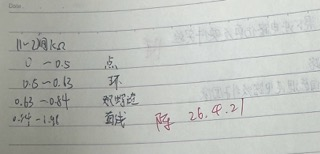
\includegraphics[scale=0.35]{签名2.jpeg}
  \caption{DX2 教师签名页}
\end{figure}

\end{document}
